\documentclass[letterpaper,11pt]{article}

\usepackage{latexsym}
\usepackage[empty]{fullpage}
\usepackage{titlesec}
\usepackage{marvosym}
\usepackage[usenames,dvipsnames]{color}
\usepackage{verbatim}
\usepackage{enumitem}
\usepackage[hidelinks]{hyperref}
\usepackage{fancyhdr}
\usepackage[english]{babel}
\usepackage{tabularx}
\usepackage{fontawesome5}
\usepackage{multicol}
\setlength{\multicolsep}{-3.0pt}
\setlength{\columnsep}{-1pt}
\input{glyphtounicode}

%new packages

\usepackage{fontenc}
\usepackage{amsmath}
\usepackage{amssymb}
\usepackage{graphicx}



%----------FONT OPTIONS----------

\pagestyle{fancy}
\fancyhf{} % clear all header and footer fields
\fancyfoot{}
\renewcommand{\headrulewidth}{0pt}
\renewcommand{\footrulewidth}{0pt}

% Adjust margins
\addtolength{\oddsidemargin}{-0.6in}
\addtolength{\evensidemargin}{-0.5in}
\addtolength{\textwidth}{1.19in}
\addtolength{\topmargin}{-.7in}
\addtolength{\textheight}{1.4in}

\urlstyle{same}

\raggedbottom
\raggedright
\setlength{\tabcolsep}{0in}

% Sections formatting
\titleformat{\section}{
  \vspace{-4pt}\scshape\raggedright\large\bfseries
}{}{0em}{}[\color{black}\titlerule \vspace{-5pt}]



% Ensure that generate pdf is machine readable/ATS parsable
\pdfgentounicode=1

%-------------------------
% Custom commands
\newcommand{\resumeItem}[1]{
  \item\small{
    {#1 \vspace{-2pt}}
  }
}

\newcommand{\classesList}[4]{
    \item\small{
        {#1 #2 #3 #4 \vspace{-2pt}}
  }
}

\newcommand{\resumeSubheading}[4]{
  \vspace{-2pt}\item
    \begin{tabular*}{1.0\textwidth}[t]{l@{\extracolsep{\fill}}r}
      \textbf{#1} & \textbf{\small #2} \\
      \textit{\small#3} & \textit{\small #4} \\
    \end{tabular*}\vspace{-7pt}
}

\newcommand{\resumeSubSubheading}[2]{
    \item
    \begin{tabular*}{0.97\textwidth}{l@{\extracolsep{\fill}}r}
      \textit{\small#1} & \textit{\small #2} \\
    \end{tabular*}\vspace{-7pt}
}

\newcommand{\resumeProjectHeading}[2]{
    \item
    \begin{tabular*}{1.001\textwidth}{l@{\extracolsep{\fill}}r}
      \small#1 & \textbf{\small #2}\\
    \end{tabular*}\vspace{-7pt}
}


\newcommand{\resumeSubItem}[1]{\resumeItem{#1}\vspace{-4pt}}

\renewcommand\labelitemi{$\vcenter{\hbox{\tiny$\bullet$}}$}
\renewcommand\labelitemii{$\vcenter{\hbox{\tiny$\bullet$}}$}

\newcommand{\resumeSubHeadingListStart}{\begin{itemize}[leftmargin=0.0in, label={}]}
\newcommand{\resumeSubHeadingListEnd}{\end{itemize}}
\newcommand{\resumeItemListStart}{\begin{itemize}}
\newcommand{\resumeItemListEnd}{\end{itemize}\vspace{-5pt}}


\begin{document}
\fontfamily{cmr}\selectfont
\begin{center}
\parbox{3.0cm}{%
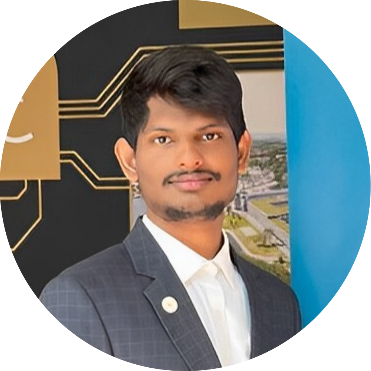
\includegraphics[width=2.7cm,clip]{images/resume_pic_m.png}}
}
\parbox{\dimexpr\linewidth-3.8cm\relax}{
\vspace{-20pt}
\begin{tabularx}{\linewidth}{L r} \\
    {\Huge \scshape  Venkata Sai Yakkshit Reddy Asodi}~
    \href{https://www.cedzlabs.com/yakkshit}{\vspace{1pt}}\\
      Berlin, Germany. \\ \vspace{1pt}
     \small \raisebox{-0.1\height}\faPhone\ +91 8179936156 ~ \href{mailto:saiyakkshit2001@gmail.com}{\raisebox{-0.2\height}\faEnvelope\  {saiyakkshit2001@gmail.com}} ~ 
    \href{https://linkedin.com/in/yakkshit/}{\raisebox{-0.2\height}\faLinkedin\ {yakkshit}}  ~
    \href{https://yakkshit.com/}{\raisebox{-0.2\height}\faGlobe\ {yakkshit.com}}  ~
    \href{https://github.com/yakkshit}{\raisebox{-0.2\height}\faGithub{ yakkshit}}
    \vspace{-8pt}
\end{tabularx}
}
\end{center}

\vspace{-23pt}
%-----------SUMMARY-----------
\href{https://www.yakkshit.com/#details}{\section{Summary \faLink}
Full Stack Developer with expertise in Vue.js and TypeScript, specializing in offline-first web applications and data processing systems. Experienced in developing responsive applications with focus on scalability and maintainability. Passionate about leveraging technology to create sustainable solutions and tackle climate change challenges.}

%-----------TECHNICAL SKILLS-----------
\section{\href{https://www.linkedin.com/in/yakkshit/details/skills/}{Technical Skills} \faLink}
\begin{itemize}[leftmargin=0.15in, label={}]
\small{\item{
\textbf{Frontend - }{Vue.js 3, TypeScript, Tailwind CSS, IndexedDB, React} \\
\textbf{Backend - }{NestJS, Node.js, SQL, RESTful APIs} \\
\textbf{DevOps \& Tools - }{Docker, Git, CI/CD, Google Cloud Platform} \\
\textbf{Data Processing - }{Time Series Data, Machine Learning Pipelines}\\
}}
\end{itemize}
\vspace{-10pt}

%-----------EXPERIENCE-----------
\section{Experience \faLinkedin}
\resumeSubHeadingListStart

\resumeSubheading
{\large Circleup AG \faBuilding}{December 2023 -- July 2024}
{Lead Full Stack Engineer}{\faMapMarker \hspace{0.1cm} Zurich, Switzerland}\\
\vspace{10pt}
\textbf{Responsibilities:}
\resumeItemListStart
\vspace{-10pt}
\resumeItem{Architected and implemented offline-first web applications using Vue.js and IndexedDB, ensuring seamless operation in low-connectivity environments.}
\resumeItem{Developed data processing pipelines for real-time sensor data, implementing efficient time-series data storage and analysis solutions.}
\resumeItem{Led the implementation of automated ML pipelines for data processing, improving system efficiency by 40\%.}
\resumeItemListEnd
\vspace{-3pt}
\textbf{Environment:}\emph{Vue.js, TypeScript, NestJS, SQL, Docker, GCP}

\resumeSubheading
{Cedzlabs \faBuilding}{March 2023 -- July 2024}
{Full Stack Developer}{\faMapMarker \hspace{0.1cm} India}\\
\vspace{10pt}
\textbf{Responsibilities:}
\vspace{-10pt}
\resumeItemListStart
\resumeItem{Built scalable web applications using Vue.js and TypeScript, focusing on maintainable architecture and code quality.}
\resumeItem{Implemented responsive UI components with Tailwind CSS and integrated real-time data processing features.}
\resumeItemListEnd
\vspace{-3pt}
\textbf{Environment:}\emph{Vue.js, TypeScript, Tailwind CSS, Node.js, Git}

\resumeItem{\textbf{\href{https://linkedin.com/in/yakkshit}{Checkout my other experiences by clicking here}}}
\vspace{-5pt}

%-----------PROJECTS-----------
\section{Projects \faGithub}
\vspace{-5pt}
\resumeSubHeadingListStart
\resumeProjectHeading
{\textbf{\href{https://ui.cedzlabs.com/resume}{Industrial IoT Dashboard}} $|$ \emph{Vue.js, TypeScript, TimescaleDB}}{2023}\\
\vspace{6pt}
\textbf{Description:}
\vspace{-5pt}
\resumeItemListStart
\resumeItem{Developed a comprehensive IoT monitoring system using Vue.js and TypeScript, featuring offline-first capabilities and real-time sensor data processing. Implemented time series data storage using TimescaleDB and created automated ML pipelines for data analysis.}
\resumeItemListEnd
\vspace{4pt}
\textbf{Tools:}\emph{Vue.js, TypeScript, TimescaleDB, IndexedDB, ML Pipelines}
\vspace{-10pt}

\resumeProjectHeading
{\href{https://yakkshit.com}{\textbf{Environmental Data Platform}} $|$ \emph{NestJS, Vue.js}}{2023}\\
\vspace{6pt}
\textbf{Description:}
\vspace{-5pt}
\resumeItemListStart
\resumeItem{Created a platform for environmental data collection and analysis using NestJS and Vue.js. Implemented containerized microservices architecture and automated CI/CD pipelines using GitHub Actions.}
\resumeItemListEnd
\vspace{4pt}
\textbf{Tools:}\emph{NestJS, Vue.js, Docker, GitHub Actions}
\vspace{-12pt}

\section{Languages}
\resumeSubHeadingListStart
\resumeSubheading
{Bachelor of Technology in Computer Science}{2019 -- 2023}
{Major in Software Engineering}{}
\resumeSubHeadingListEnd

\section{Achievements / Professional Development}
\resumeSubHeadingListStart
\resumeItemListStart
\resumeItem{Implemented offline-first architecture patterns, reducing data sync conflicts by 60\%.}
\resumeItem{Contributed to open-source Vue.js components and time-series data processing libraries.}
\resumeItem{Active participant in climate tech meetups and sustainable technology workshops.}
\resumeItemListEnd

\resumeSubHeadingListEnd
\textbf{Strengths:}\emph{Problem-solving, attention to detail, sustainable development focus, adaptability} \\
\textbf{Languages:}\emph{Telugu - Native $|$ English - Fluent $|$ Hindi - Fluent $|$ German - Elementary $|$ Swedish - Elementary.}

\vspace{10pt}
\end{document}